A halfedge data structure \cite{Weiler:1985:EDS} is an edge-centered data
structure capable of maintaining incidence informations of vertices,
edges and faces, for planar maps, polyhedron, or other orientable,
two-dimensional surfaces embedded in arbitrary dimension. Each edge is
decomposed into two halfedges with opposite orientations.  Two types
of halfedge can be chosen for the data structure: facet-edge pair or
vertex-edge pair. One incident face and one incident vertex are
stored in each halfedge. For each face and each vertex, one incident
halfedge is stored (see Fig.\ref{fig:halfedge}). The halfedge is
designated as the connectivity primitive. Connectivity manipulations
are based on the reconfiguration and the mesh traversal is equivalent
to the adjacency walking of the halfedges. Halfedge data structures
have been very successful for the design of algorithms on meshes for
several reasons:
\begin{itemize}
\item halfedges contain a constant number of adjacencies. 
\item halfedges encode the mesh orientation.
\item navigation around vertices or facets is easy.
\item corner attributes, such as crease normals, is allowed 
      to be associated with halfedges.
\end{itemize}

\begin{figure}[htb]
    \centering{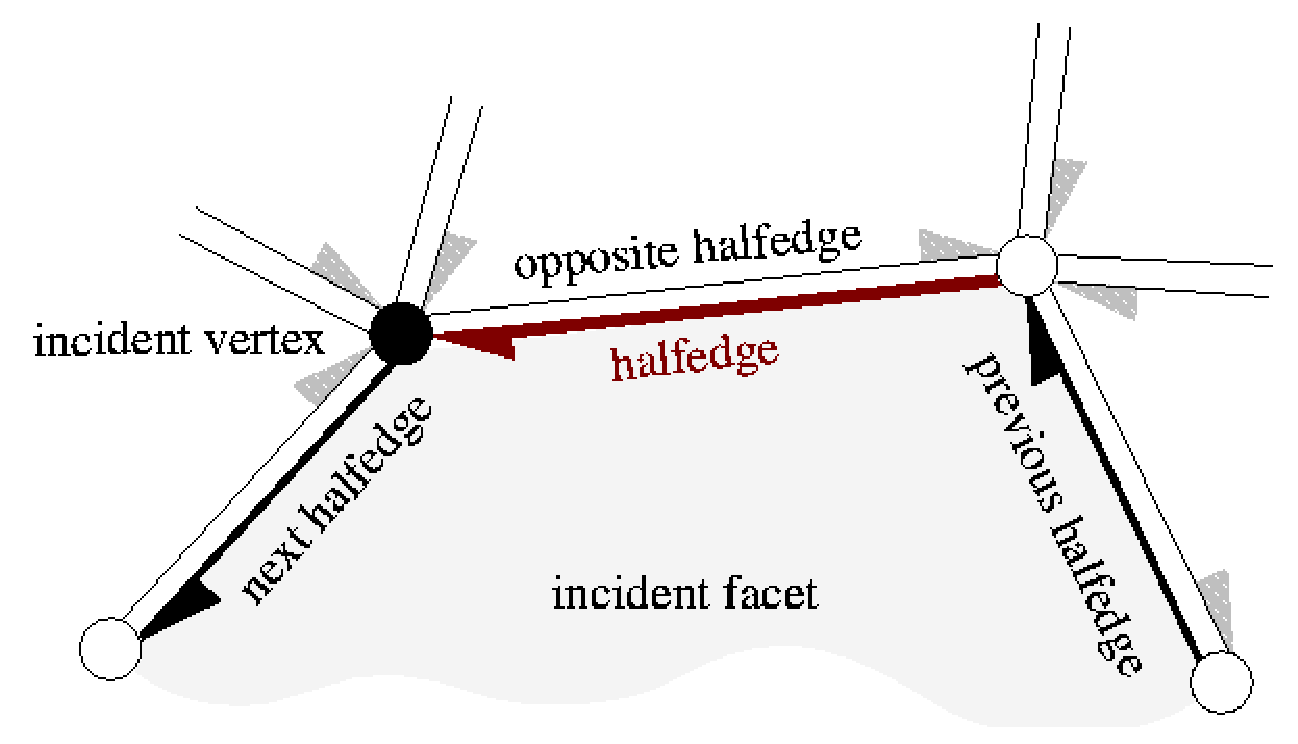
\includegraphics[width=5.0cm]{figs/halfedge}}
    \caption{One halfedge and its incident primitives.}
    \label{fig:halfedge}
\end{figure}

%% Halfedge data structure is a combinatorial data structure.  The
%% geometric interpretation is instantiated with a defined kernel. A
%% geometry kernel defines the dimensional primitives such as points and
%% vectors and the geometry metrics such as distances and angles. A
%% polyhedron is a constrained combinatorial structure that can only
%% represent a 2-manifold. A 2-manifold is a surface where every point is
%% embedded by a disk (interior points) or a half disk (boundary
%% points). Polyhedrons are usually interpreted as the shell of a solid
%% bounded by plane polygons in the 3D Euclidean space.

%% In the \poly, the \hds\ is interfaced and indirectly manipulated
%% by the \poly. Since \hds\ is the internal representation of the
%% connectivity structure, primitives traversal of the \poly\ is
%% supported by the \hds . As a container, the \hds\ provides 
%% iterators of the primitives, i.e. vertices, halfedges and faces.
%% This primitive iterators visit the primitives on the storage
%% order of the internal list or vector. As a connected graph,
%% the \hds\ provides circulators around vertices or faces.
%% The circulator visits the halfedges adjacent to the vertex
%% in CW order and the face in CCW order. Details of using iterators
%% and circulators can be found at \ref{sec:??}.

%% Halfedges in a \hds\ also provide a set of low-level 
%% traversal operators. These operators include the prev(), next(), 
%% opposite(), vertex(), and face(). The prev(), next() and opposite()
%% return the handle of the previous, next and opposite
%% halfedge respectively. The vertex() returns the handle of the 
%% incidence vertex and the face() returns the handle of the 
%% incidence face. The next() and opposite() are mandatory and others
%% are optionally support. Though in this tutorial, a complete
%% support is assumed. For how to define a partially support \hds ,
%% readers should refer to \cite{cgalmanul}.   


